%%%%%%%%%%%%%%%%%%%%%%%%%%%%%%%%%%%%%%%%%%%%%%%%%%%%%%%%%%%%%%%%%%%%
% Ergebnisse
%%%%%%%%%%%%%%%%%%%%%%%%%%%%%%%%%%%%%%%%%%%%%%%%%%%%%%%%%%%%%%%%%%%%
\chapter{Results}
  \label{results}

% \todo{
% In this chapter which also could be more than one chapter, depending on the nature of the thesis, the results of the thesis are presented.
% Make sure you illustrate your results with appropriate figures and tables, but do not discuss the results here. This should be done in a separate discussion chapter.
% Or maybe do combine results and discussion and split by research questions.
% }
\section{Discretization}
\begin{figure}[h]
  \centering
  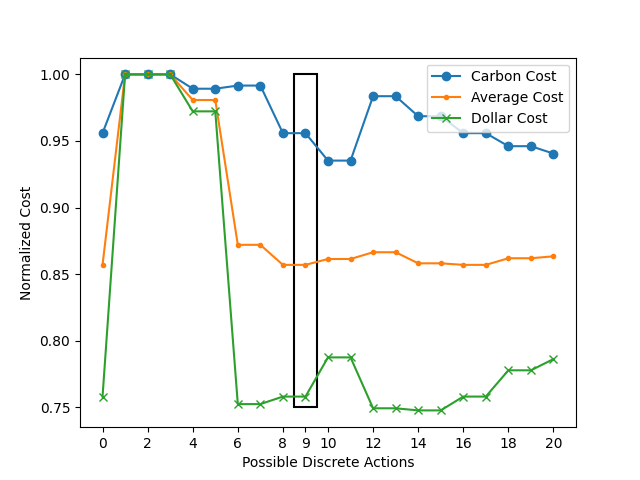
\includegraphics[width=\figurewidth]{figures/discretization.png}
  \caption{This graph shows the effect of the discretization resolution on the rule-based control algorithm. The coarsest resolution that does not significantly impact performance and includes the zero action is 9. In this graph, 0 possible actions means no discretization is applied.}
  \label{fig:discretization}
\end{figure}

The results from the pre-experiment on the effect of discretization are shown in figure \ref{fig:discretization}.
The rule-based agent performs comparably to the continuous case when discretization resolution is high, and worse on coarse resolutions. The coarsest resolution that performs similarly well as the continuous case is the subdivision into 8 or 9 possible actions.

\section{Hyperparameter Tuning}
All 200 runs of $\epsilon$-greedy DQN completed successfully.
10/100 runs of UA-DQN, all runs with a batch size of 1, failed.
18/200 runs of DQN-Softmax failed, all of which share a batch size of 8.
However, 17 other runs with a batch size of 8 completed successfully.

Table \ref{tab:hyperparameters} shows the results of the tuning process for each algorithm.
For each algorithm, the learning rate had the most significant correlation with final performance, followed by the batch size and the target network update frequency.
The $\epsilon$ parameter of the optimizer Adam showed a large effect only for $\epsilon$-greedy DQN.

Figure \ref{fig:tuning_results} shows a histogram of the final performance of all successful tuning runs.
52\% of all UADQN runs perform better than the idle policy, 40.5\% of all DQN-Softmax  runs perform better than the idle policy, and 37\% of e-greedy DQN runs perform better than the idle policy.

Both DQN algorithms show a peak at around -5000, which corresponds to strategies that are close to the idle policy.

\begin{table}[h]
  \centering
  \caption{This Table shows the correlation between tuned hyperparameters and algorithm performance for successful runs.}
  \label{tab:hyperparameters}
  \begin{tabular}{c||c|c|c}
    Algorithm & Hyperparameter & Value for Best Run & \makecell{Correlation with \\ final score} \\ \hline 
    UA-DQN & Learning Rate                                & 3e-4 & \bf{-0.47}\\
           & Batch Size                                   & 128 &  0.28\\
           & Adam's $\epsilon$                            & 1e-07 & -0.03\\
           & \makecell{Update Frequency \\of Target Network }& 4 & -0.11\\ \hline
    DQN-Softmax & Learning Rate                                 & 3e-4 & \bf{-0.36} \\
                & Batch Size                                    & 128 & -0.18\\
                & Adam's $\epsilon$                             & 1e-05 & -0.02\\
                & \makecell{Update Frequency \\of Target Network } & 4 &  0.16\\ \hline
    $\epsilon$-greedy DQN & Learning Rate                       & 7e-05 & \bf{-0.33}\\
                & Batch Size                                    & 4 & -0.19\\
                & Adam's $\epsilon$                             & 1e-08 &  0.10\\
                & \makecell{Update Frequency \\of Target Network } & 16 &  0.14

  \end{tabular}
\end{table}



\begin{figure}
  \centering
  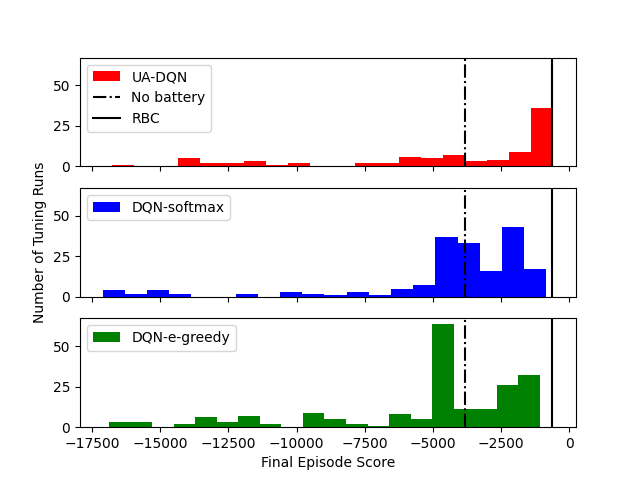
\includegraphics[width=\figurewidth]{figures/tuning_results.png}
  \caption{This histogram shows the final episode reward of all successful tuning runs. Every run represents one choice for the hyperparameters. The performance of the rule-based controller and the idle policy are shown for reference.}
  \label{fig:tuning_results}
\end{figure}

\section{Comparison of Tuned Algorithms}
\begin{figure}
  \centering
  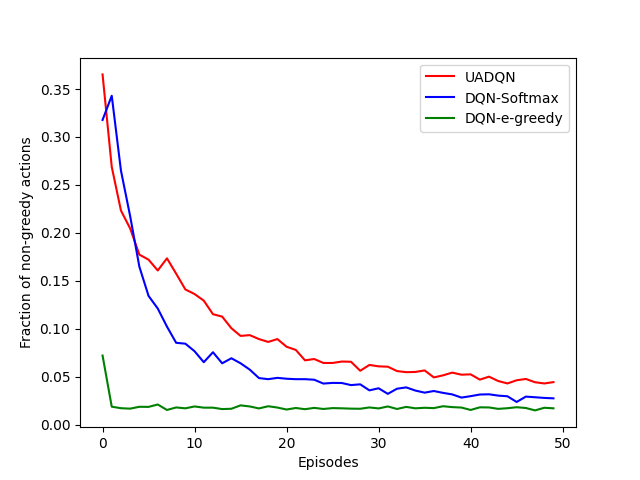
\includegraphics[width=\figurewidth]{figures/non-greedy-fraction.png}
  \caption{This graphic shows the exploration rate of tuned algorithms throughout the training process. It highlights the different action selection strategies employed by the different algorithms. UA-DQN keeps exploring more than the other strategies.}
  \label{fig:non_greedy_fraction}
\end{figure}
To illustrate the difference in exploration between the algorithms, figure \ref{fig:non_greedy_fraction} shows the fraction of selected non-greedy actions per episode.
All algorithms start out exploring more and then gradually decrease their exploration rate.
DQN-Softmax and UA-DQN explore more than $\epsilon$-greedy DQN, which quickly reaches an exploration rate of $\epsilon = 0.02$.
UA-DQN keeps exploring more than the other algorithms.

Figure \ref{fig:tuning_validation} shows the episode rewards of the selected hyperparameters for each algorithm during training.
Tuned UA-DQN converges faster than the other algorithms, and it converges to a better mean performance, as shown in table \ref{tab:tuned_results}. The hand-engineered rule-based agent outperforms the tuned reinforcement learning algorithms on both metrics.

When repeated with 10 different seeds, a single run of DQN-Softmax failed, compared to no failures from the other algorithms.


\begin{figure}
  \centering
  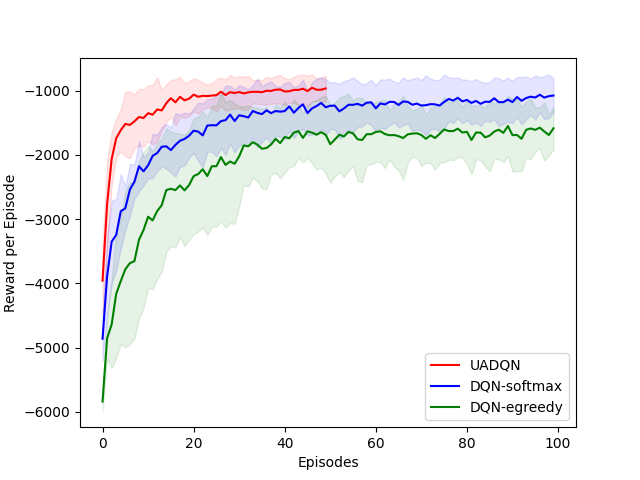
\includegraphics[width=\figurewidth]{figures/tuning_validation.png}
  \caption{This graphic shows the performance during training of the three tuned algorithms. The shaded area shows the standard deviation over 10 runs with different random seeds. Tuned UA-DQN converges after fewer episodes than either DQN variant. UA-DQN was only trained for 50 episodes due to the larger resource requirements of the algorithm.}
  \label{fig:tuning_validation}
\end{figure}

\begin{table}
  \centering
  \caption{This table shows the mean time per training episode for each of the tuned algorithms.}
  \label{tab:resources}
  \begin{tabular}[pos]{c|c}
    Agent & Mean Time per Training Episode \\ \hline           
    UA-DQN   & 95.3s \\
    DQN-Softmax  &27.2s \\
    $\epsilon$-greedy DQN &20.7s \\
  \end{tabular}
\end{table}

\begin{table}
  \centering
  \caption{This table shows the mean performance of tuned algorithms when evaluated using their respective action selection policy for one episode on Building 1. I also give the standard deviation of the combined average.}
  \label{tab:tuned_results}
  \begin{tabular}{l|ccccc}
    Agent                 & Dollar Cost & Carbon Emission & Average \\ \hline
    Control (Idle)   & 1    & 1    & \textbf{1}    \\
    $\epsilon$-greedy DQN & 0.83 & 0.94 & $\mu = \mathbf{0.88}, SD = 0.017$ \\
    DQN-Softmax           & 0.83 & 0.93 & $\mu = \mathbf{0.88}, SD = 0.019$ \\
    UA-DQN                & 0.82 & 0.91 & $\mu = \mathbf{0.87}, SD = 0.010$ \\
    Discrete Rule-Based   & 0.80 & 0.88 & \textbf{0.84}
  \end{tabular}
\end{table}
